\documentclass[tikz,border=10pt]{standalone}
\usepackage{amsmath}
\usepackage{amssymb}
\usepackage{tikz}
\usetikzlibrary{arrows.meta,calc}

\definecolor{figazul}{RGB}{2,132,199}
\definecolor{figrojo}{RGB}{220,38,38}
\definecolor{figverde}{RGB}{22,163,74}

\begin{document}
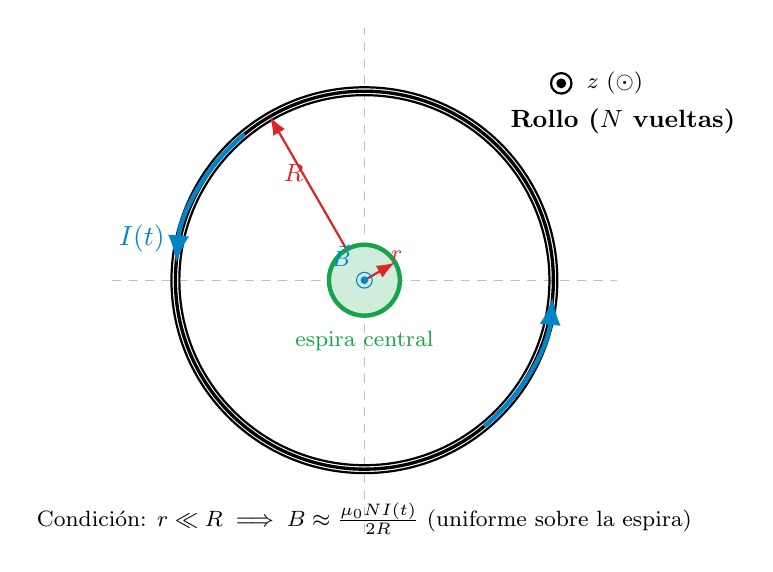
\begin{tikzpicture}[>=Latex, line cap=round, line join=round]
  % Ejes tenues
  \draw[dashed, color=gray!50] (-3.2, 0) -- (3.2, 0);
  \draw[dashed, color=gray!50] (0, -3.2) -- (0, 3.2);

  % Rollo plano de N vueltas circulares de radio R = 2.4
  % Se dibujan varias vueltas concéntricas muy próximas para dar la idea visual de rollo de alambre
  \draw[thick] (0, 0) circle (2.35);
  \draw[very thick] (0, 0) circle (2.40);
  \draw[thick] (0, 0) circle (2.45);
  \node[above right, font=\small\bfseries] at (45:2.45) {Rollo ($N$ vueltas)};

  % Flecha de corriente I(t) en sentido antihorario
  \draw[->, ultra thick, color=figazul] (130:2.4) arc (130:175:2.4) node[above left, color=figazul] {$I(t)$};
  \draw[->, ultra thick, color=figazul] (-50:2.4) arc (-50:-5:2.4);

  % Cota del radio R del rollo (en rojo)
  \draw[->, thick, color=figrojo] (0, 0) -- (120:2.4);
  \node[above left, color=figrojo, font=\small] at (120:1.3) {$R$};

  % Pequeña espira circular concéntrica de radio r (r << R)
  \draw[ultra thick, color=figverde, fill=figverde!20] (0, 0) circle (0.45);
  \node[below=2pt, font=\footnotesize, color=figverde] at (0, -0.45) {espira central};

  % Cota del radio r de la pequeña espira (en rojo)
  \draw[->, thick, color=figrojo] (0, 0) -- (30:0.45);
  \node[above right, color=figrojo, font=\footnotesize] at (30:0.25) {$r$};

  % Campo B producido en el centro (\odot saliente, azul)
  \draw[thin, color=figazul] (0, 0) circle (0.10);
  \fill[color=figazul] (0, 0) circle (1.4pt);
  \node[above left, font=\footnotesize, color=figazul] at (-0.05, 0.05) {$\vec{B}$};

  % Eje z perpendicular saliente
  \draw[thick] (2.5, 2.5) circle (0.13);
  \fill (2.5, 2.5) circle (1.8pt);
  \node[right, font=\footnotesize] at (2.7, 2.5) {$z$ ($\odot$)};

  % Condición geométrica y fórmula
  \node[below, font=\footnotesize, align=center] at (0, -2.7) {Condici\'on: $r \ll R \implies B \approx \frac{\mu_0 N I(t)}{2R}$ (uniforme sobre la espira)};

\end{tikzpicture}
\end{document}
